%%% In this section, you will describe all of the various artifacts that you will generate and maintain during the project life cycle. Describe the purpose of each item below, how the content will be generated, where it will be stored, how often it will be updated, etc. Replace the default text for each section with your own description. Reword this paragraph as appropriate.

\subsection{Major Documentation Deliverables}

\subsubsection{Project Charter}
This document will be updated every sprint to reflect any changes the project may encounter. The changes may include: additional equipment/expenditures, added/removed functionality, etc. The initial version of this charter will be delivered Monday, October 1st and the final version will be delivered at the end of Senior Design II along with the final product.

\subsubsection{System Requirements Specification}
The system requirements specification will be be completed by the end of the second sprint on October 23rd. Any changes will be approved by team agreement, and the final version will be turned in along with the final product.

\subsubsection{Architectural Design Specification}
The architectural design specification document will be updated any time the team agrees that it needs to be changed. Any member may propose changes via Slack, and the team will discuss whether the change is appropriate and required. The Product Owner will be the final authority on changes to this document. The initial version will be completed by the end of Sprint \#3, on November 13th, and the final version will be part of the completed project.

\subsubsection{Detailed Design Specification}
The detailed design specification will be updated with each sprint, to match the reality of the project. This document will be completed next semester, exact dates not yet finalized.

\subsection{Recurring Sprint Items}

\subsubsection{Product Backlog}
Items from the SRS will be added to the product backlog based on how the overall architecture of the app is laid out. For example, requirements dealing with the interfaces to the OctoPrint and Google Cloud Speech APIs would be some of the first items to be added to the product backlog. These decisions will be decided by a team vote and the product backlog will be maintained/shared as an Excel spreadsheet on the team's Google Drive.

\subsubsection{Sprint Planning}
In each sprint, the whole team will meet for approximately one hour per week to plan the next sprint. In this meeting, they will agree to complete a number of items from the product backlog during the next sprint. Based on the results of this meeting, a sprint backlog will be defined for the next sprint. The sprint backlog will be incorporated into the sprint plan. The project will consist of 8 sprints (4 sprints in Senior Design I and 4 sprints in Senior Design II).

\subsubsection{Sprint Goal}
The development team will decide the sprint goal for each sprint by majority vote with the advice of the scrum master. Based on the customer's requirements, the Product Owner will list the objectives that the sprint should achieve. Then, the development team will select items from the product backlog that help meet the sprint goal. 

\subsubsection{Sprint Backlog}
The development team will decide which product backlog items are incorporated into the sprint backlog for each sprint. The sprint backlog will be maintained/shared as an Excel spreadsheet on the team's Google Drive. 

\subsubsection{Task Breakdown}
Individual tasks from the sprint backlog may be assigned in one of two ways: 
\begin{itemize}

\item If the tasks are of equal difficulty, as determined by the Scrum Master, then any team member may voluntarily claim that task.

\item If some tasks are more difficult than others, as determined by the Scrum Master, then a team member may claim them if and only if he is technically competent in that area or has demonstrated a willingness to learn how to perform that task. 

\item If the Scrum Master decides that a task is too large for one team member to complete within the allotted time, then he will divide it into multiple sub tasks and these will be assigned as stated above. Optionally, two team members may elect to work together on the task. 

\end{itemize}
Depending on the end date of each sprint, team members will estimate the time that they think they will need to complete their tasks. Note: Each member's estimated task completion date must be earlier than the end date. 

\subsubsection{Sprint Burn Down Charts}
For each sprint, team members will keep updating the "Status" column for their assigned tasks. As long as the "Status" column is updated to "Finished", the sprint burn down chart will be updated and generated automatically. 

The total amount of effort expended by each individual team member may be accessed as follows:

\begin{itemize}
    
\item In a sprint backlog spreadsheet, click on the "Assigned to" column to see the tasks that have been assigned to each member and click on the "Status" column to see which of these tasks have been completed. 

\end{itemize}
The sprint burn down chart will be formatted as a release burn down chart.
An example of a sprint burn down chart chart is shown in Figure 2 on the next page.

\begin{figure}[h!]
	\centering
   	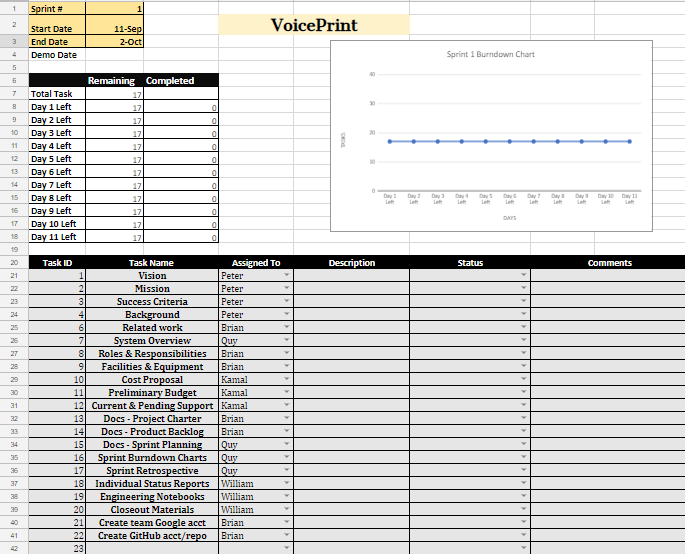
\includegraphics[width=0.6\textwidth]{images/Chart.png}
    \caption{Example sprint burn down chart}
\end{figure}

\newpage\subsubsection{Sprint Retrospective}
For each sprint, with the presentation of all team members, the team will firstly schedule a sprint review, then the team will schedule a sprint retrospective. The team will choose the time that is best fit for all team members. If the sprint review was good, the team would have discussion about sprint retrospective. Each task will be documented as individuals. After the group reviewing, all the tasks will be putting together as a single document before turning in as group. Each team has different due day for team assignment. In our team, we decide to have everything get done at least 3 days before the due day of the sprint.

\subsubsection{Individual Status Reports}
For every sprint, all group members will submit an individual status report. This report will show an individual's status on a given sprint (behind, ahead, etc). Some key items included in the status report include: the sprint goal, backlog, logged hours, burnout chart, and individual retrospective.

\subsubsection{Engineering Notebooks}
The engineering notebooks will be updated once a week at a minimum by each team member and each update will consist of one page. To maintain accountability, the team will meet before and/or after class every Monday and Wednesday. Currently the team plans on having no designated "witness" for the notebooks; therefore, the "witness" for each engineering notebook page will vary based on who was present when the notebook was being updated.

\subsection{Closeout Materials}

\subsubsection{System Prototype}
The \textit{VoicePrint} system prototype will be an operational app installable to Android devices that allows a user to print a 3D object using voice commands. It will be demonstrated in the Senior Design Lab.

\subsubsection{Project Poster}
The project poster will be 3' x 3' and include information about 3D printing in general, how \textit{VoicePrint} works, and have pictures of the application and at least one finished object printed by voice commands.

\subsubsection{Web Page}
The project web page will include a walkthrough of application functionality. Each option will be explained and a tutorial will be available to help new users utilize the app. Source code documentation will be included on one page.

\subsubsection{Demo Video}
The demo video will show how the app works. The video will show step-by-step how the app operates, beginning from the setup and ending with a finished 3D printed object. The video will be at most 5 minutes.

\subsubsection{Source Code}
\textit{VoicePrint} source code will be maintained on GitHub, which provides version control as well. No source will be provided to end users.  Inside the application will be an "about" option that lists any relevant licenses used.

\subsubsection{Source Code Documentation}
Doxygen will be used for source code documentation. The final documentation will be exported to the web page.

\subsubsection{Installation Scripts}
Installation will be performed by simply installing the final .apk to an end user's Android device. No additional considerations for servers should be necessary, as the only external communication required will be handled by API calls to Google or Amazon.

\subsubsection{User Manual}
A user manual will be provided in the app displayed as a help button. Setup as well as instructions on how to operate the app will be located here.
